% yaml_architecture.tex
% Complete architecture diagram showing internal structure
% Author: João Pedro Azevedo
% Date: December 2025

\documentclass[tikz,border=10pt]{standalone}
\usepackage{tikz}
\usetikzlibrary{shapes.geometric, arrows.meta, positioning, fit, backgrounds, calc, patterns}

\begin{document}

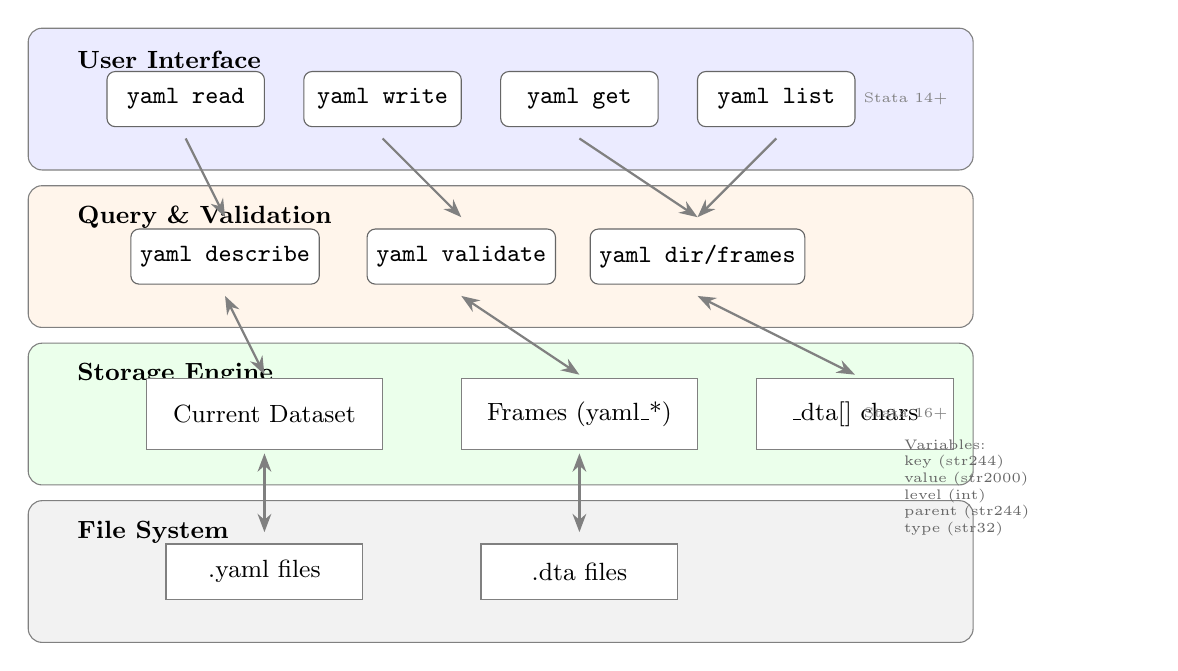
\begin{tikzpicture}[
    % Layer styles
    layer/.style={
        rectangle, 
        rounded corners=5pt,
        draw=black!50, 
        minimum width=12cm,
        minimum height=1.8cm,
        font=\small
    },
    % Component box
    compbox/.style={
        rectangle, 
        rounded corners=3pt,
        draw=black!60, 
        fill=white,
        minimum width=2cm, 
        minimum height=0.7cm,
        font=\small\ttfamily
    },
    % Arrow style
    arrow/.style={
        ->,
        >=Stealth,
        thick,
        black!50
    },
    biarrow/.style={
        <->,
        >=Stealth,
        thick,
        black!50
    }
]

% === Layer 1: User Interface (Top) ===
\node[layer, fill=blue!8] (ui) at (0, 6) {};
\node[font=\small\bfseries, anchor=west] at (-5.5, 6.5) {User Interface};

\node[compbox] at (-4, 6) {yaml read};
\node[compbox] at (-1.5, 6) {yaml write};
\node[compbox] at (1, 6) {yaml get};
\node[compbox] at (3.5, 6) {yaml list};

% === Layer 2: Query & Validation ===
\node[layer, fill=orange!8] (query) at (0, 4) {};
\node[font=\small\bfseries, anchor=west] at (-5.5, 4.5) {Query \& Validation};

\node[compbox] at (-3.5, 4) {yaml describe};
\node[compbox] at (-0.5, 4) {yaml validate};
\node[compbox] at (2.5, 4) {yaml dir/frames};

% === Layer 3: Storage Engine ===
\node[layer, fill=green!8] (storage) at (0, 2) {};
\node[font=\small\bfseries, anchor=west] at (-5.5, 2.5) {Storage Engine};

\node[rectangle, draw=black!50, fill=white, minimum width=3cm, minimum height=0.9cm] 
    (dataset) at (-3, 2) {\small Current Dataset};
\node[rectangle, draw=black!50, fill=white, minimum width=3cm, minimum height=0.9cm] 
    (frames) at (1, 2) {\small Frames (yaml\_*)};
\node[rectangle, draw=black!50, fill=white, minimum width=2.5cm, minimum height=0.9cm] 
    (chars) at (4.5, 2) {\small \_dta[] chars};

% === Layer 4: File System ===
\node[layer, fill=gray!10] (fs) at (0, 0) {};
\node[font=\small\bfseries, anchor=west] at (-5.5, 0.5) {File System};

\node[rectangle, draw=black!50, fill=white, minimum width=2.5cm, minimum height=0.7cm] 
    (yamlfiles) at (-3, 0) {\small .yaml files};
\node[rectangle, draw=black!50, fill=white, minimum width=2.5cm, minimum height=0.7cm] 
    (dtafiles) at (1, 0) {\small .dta files};

% === Arrows between layers ===
\draw[arrow] (-4, 5.5) -- (-3.5, 4.5);
\draw[arrow] (-1.5, 5.5) -- (-0.5, 4.5);
\draw[arrow] (1, 5.5) -- (2.5, 4.5);
\draw[arrow] (3.5, 5.5) -- (2.5, 4.5);

\draw[biarrow] (-3.5, 3.5) -- (-3, 2.5);
\draw[biarrow] (-0.5, 3.5) -- (1, 2.5);
\draw[biarrow] (2.5, 3.5) -- (4.5, 2.5);

\draw[biarrow] (-3, 1.5) -- (-3, 0.5);
\draw[biarrow] (1, 1.5) -- (1, 0.5);

% === Version annotations ===
\node[font=\tiny, text=black!50, anchor=east] at (5.8, 2) {Stata 16+};
\node[font=\tiny, text=black!50, anchor=east] at (5.8, 6) {Stata 14+};

% === Data model annotation ===
\node[font=\tiny, text=black!60, anchor=north west, text width=3cm] at (5, 1.8) {
    Variables:\\
    key (str244)\\
    value (str2000)\\
    level (int)\\
    parent (str244)\\
    type (str32)
};

\end{tikzpicture}

\end{document}
